\documentclass[]{beamer}


\title{Toxicity of Mushrooms}
\author{Michael Vincent}
\institute{Coding Dojo}
\date{September 7}
\begin{document}

\maketitle

\begin{frame}
\frametitle{Business Problem}

The residents of Fungopolis have developed a keen interest in gathering their own mushrooms. The city council has grown concerned that all of this amateur mushroom foraging will result in needless death. We have been tasked with constructing a machine learning model that will predict the toxicity of a mushroom based on certain characteristics of the mushroom.
\end{frame}

\begin{frame}
\frametitle{The Data}

We used the ``Secondary Mushroom Dataset'' from the Machine Learning Repository at UCI. This is a synthetic data set with about 60,000 data points and 21 attributes. The following is a sample of the attributes included in the data set.
\pause
\begin{itemize}
\item Cap color
\item Cap diameter
\item Cap shape
\item Stem height
\item Stem width
\end{itemize}
\end{frame}


\begin{frame}
\frametitle{Visualization 1}
\begin{center}
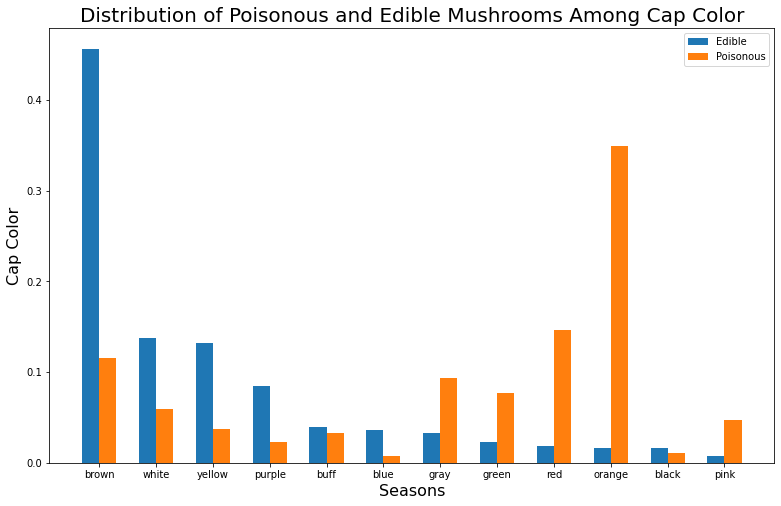
\includegraphics[scale = 0.3]{toxicity_by_color.png}
\end{center}

\pause
This graph shows that mushrooms with brown caps are more likely to be edible, while mushrooms with orange and brown caps tend to be poisonous.
\end{frame}


\begin{frame}
\frametitle{Visualization 2}
\begin{center}
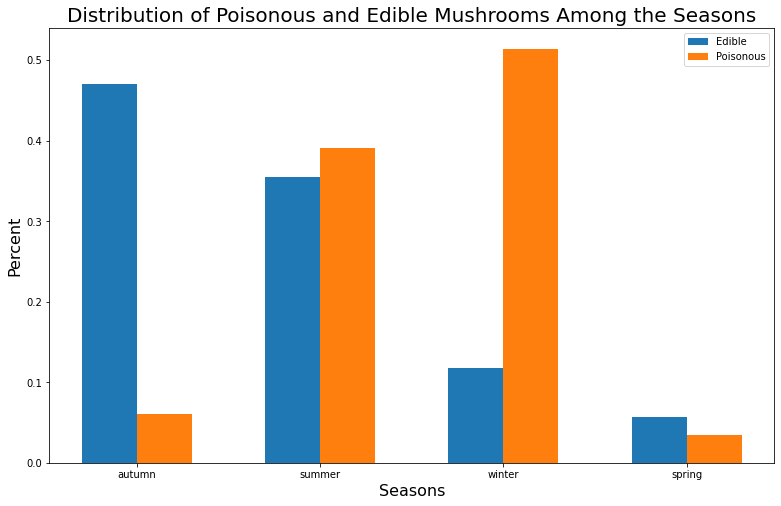
\includegraphics[scale = 0.3]{toxicity_by_season.png}
\end{center}

\pause
This graph shows that mushrooms that grow in autumn are more likely to be edible, while mushrooms that grow in winter are more likely to be poisonous.
\end{frame}


\begin{frame}
\frametitle{Model Discussion}
\begin{itemize}
\pause
\item A decision tree was used to classify mushrooms as ``edible'' or ``poisonous.'' The decision tree was chosen for its speed and metrics.
\pause
\item Model had perfect accuracy, precision, and recall. This is likely due to the fact we used a synthetic data set.
\pause
\item We could put the industrious and DIY attitude of the citizens of Fungopolis to good use and task them with gathering data for a more realistic data set. 
\pause
\item With this more realistic data set, we would not be likely to have perfect scores for our models. In this case we would want our recall to be as close to one as possible.
\pause
\item High recall means fewer false negatives. A false negative in our model means incorrectly identifying a mushroom as edible.
\end{itemize}
\end{frame}


\begin{frame}
\frametitle{Recommendations}
\begin{itemize}
\pause
\item Inexperienced mushroom foragers should only gather mushrooms in the autumn. The fewest poisonous mushrooms grow in autumn. Significant proportions of poisonous mushrooms grow in all other seasons. Poisonous mushrooms are particularly common in winter, so we recommend only the most experienced mushroom foragers gather mushrooms in winter.
\pause
\item Inexperienced mushroom foragers should only gather mushrooms with brown caps. The greatest proportion of edible mushrooms have brown caps. All other cap colors have significant proportions of poisonous mushrooms, so it is better for mushroom foragers with little experience to avoid these mushrooms.
\pause
\item If more accurate models are desired, then we recommend gathering real world data.
\pause
\item Thanks for your time!
\end{itemize}
\end{frame}
\end{document}